\def\parentDir{Topology/SimplePoincareTorusBundle}

\subsection{Simple Example of Poincare's Torus Bundles}

We will consider a simple example of a 3-manifold studied by Poincare; see Stillwell 
\cite{stillwell3Mnflds} for more information. Consider \(\mathbb R^3\) under the following equivalencies:

\begin{equation}
\begin{cases}
(x, y, z) \sim (x + 1, y, z), \\
(x, y, z) \sim (x, y + 1, z), \\
(x, y, z) \sim (x + y, y, z + 1).
\end{cases}
\end{equation}
Our manifold \(M = \mathbb R^3 / \sim\), the quotient of \(\mathbb R^3\) by these equivalencies. A fundamental domain is 
provided by the unit cube \(\{0 \leq x, y,z \leq 1\}\) (ignoring issues of which sides to include if we are absolutely insistent
as to uniqueness of representation of equivalence classes).  

We see that every horizontal slice \(\{z = c\}\) is a 2-dimensional torus. Furthermore, the slice \(\{z = 0\}\) and \(\{z = 1\}\)
is given by a glide transformation where the transformation \(T(x, y) = (x + y, x)\).

We will compute the fundamental group \(\pi_1(M)\) of this manifold by using two triangulations. The first will be a very improper
triangulation, and the second will be much more proper although a little more complex.

\subsection*{An Improper Triangulation}

First let's consider an improper triangulation/delta complex on \(M\). Pictured below are slices for this triangulation on the unit cube for
\(z = 0\), some \(0 < z < 1\), and \(z = 1\).

\begin{figure}[H]
\centering
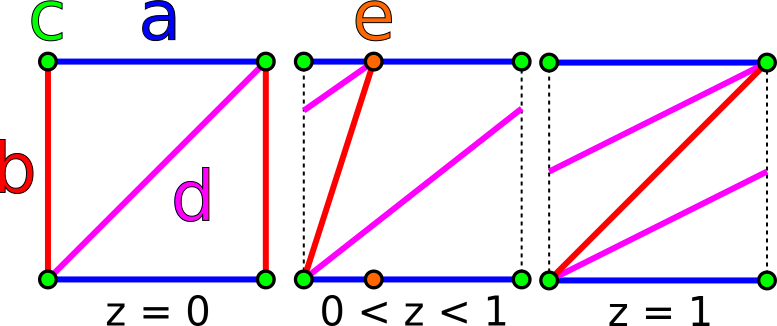
\includegraphics[width = 4in]{_generated/slices.pdf}
\end{figure}

Why is this triangulation improper? It is due to the fact that the line segment \(d\) cuts across the face represented by blue in each slice.
Now, this doesn't mean it is invalid. It is just not a proper delta-complex; it is more properly described as a CW-complex.

Let's compute \(\pi_1(M)\) using this triangulation. First, we find the generators of the fundamental group that come from this
triangulation. We need to find a minimal spanning tree inside the 1-complex of our triangulation. Let us root the tree at the
vertex that is the corner of \(\{z = \}\) of the fundamental domain; recall that all four corners are equivalent.

Next, we see that all of the 1-cells are attached to the root of the tree. Furthermore, every one cell takes the root back to itself. Therefore,
our minimal spanning tree just conists of a single vertex, the root of the tree. Therefore, every 1-cell is a generator for \(\pi_1(M)\). So
we know that \(\pi_1(M)\) is generated by \(a, b, c, d,\) and \(e\).

Now let us find the relations between these generators that come from the faces (i.e. 2-cells) of our triangulation.

The horizontal 2-cells in the slice \(\{z = 0\}\) give 
\begin{equation}
d \sim ab \sim ba. 
\end{equation}
This is expected as every horizontal slice is just a 2-dimensional torus.

Next, let us investigate the relations due to the vertical faces. So we look at each color in the \(\{0 < z < 1\}\) to see where the faces are.
Note, that the blue color is a little misleading as \(e\) cuts across this face. So let us look at this face explictly.
\begin{figure}[H]
\centering
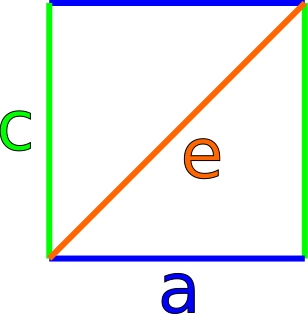
\includegraphics[width=2in]{_generated/improperVertFace.pdf}
\end{figure}
The blue face gives us
\begin{equation}
e \sim ac \sim ca.
\end{equation}
Note that we also have that \(a\) commutes with \(c\).

The red vertical face gives
\begin{equation}
beb^{-1}c^{-1} \sim 1.
\end{equation}
This allows us to solve for \(e\) in terms of \(b\) and \(c\),
\begin{equation}
e \sim b^{-1}cb.
\end{equation}

Finally, the fuschia vertical face gives
\begin{equation}
ded^{-1}c^{-1} \sim 1.
\end{equation}
Given that \(d \sim ab\), \(e\sim b^{-1}cb\), and \(a\) commutes with both \(b\) and \(c\), we get
\begin{align}
1 & \sim abb^{-1}cbb^{-1}a^{-1}c^{-1}, \\
& \sim aca^{-1}c^{-1}, \\
& \sim 1.
\end{align}
Therefore, the fuschia face hasn't given us anything new.

Our relations are thus
\begin{equation}
\begin{cases}
d \sim ab \sim ba, \\
e \sim b^{-1}cb , \\
e \sim ac \sim ca.
\end{cases}
\end{equation}
So we see that the true generators are \(a, b,\) and \(c\). Thus we see that our relations may be described more succinclty as
\begin{equation}
\begin{cases}
ab \sim ba, \\
ac \sim ca, \\
cb \sim abc.
\end{cases}
\end{equation}
The last relation tells us how to deal with changing the order of \(b\) and \(c\); in the process, we pick up an \(a\).

So let us see what happens when we take the product of powers of \(a, b,\) and \(c\). We have
\begin{align}
a^{p_1}b^{q_1}c^{r_1} a^{p_2}b^{q_2}c^{r_2} & \sim a^{p_1 + p_2} b^{q_1}c^{r_1}b^{q_2}c^{r_2}, \\
 & \sim a^{p_1 + p_2 + r_1 q_2} b^{q_1 + q_2} c^{r_1 + r_2}.  
\end{align}

So we see that we can represent \(\pi_1(M)\) by a semi-direct product
\begin{equation}
\mathbb Z^2 \rtimes_\phi \mathbb Z,
\end{equation}
where \(\phi_r(p, q) = (p + rq, q) = T^r (p, q)\), \(a = (1, 0, 0)\), \(b = (0, 1, 0)\), and \(c = (0, 0, 1)\).

\subsection*{A More Proper Triangulation}

Next, let us remark on a more proper triangulation that would also let us compute \(\pi_1(M)\). 
\begin{figure}[H]
\centering
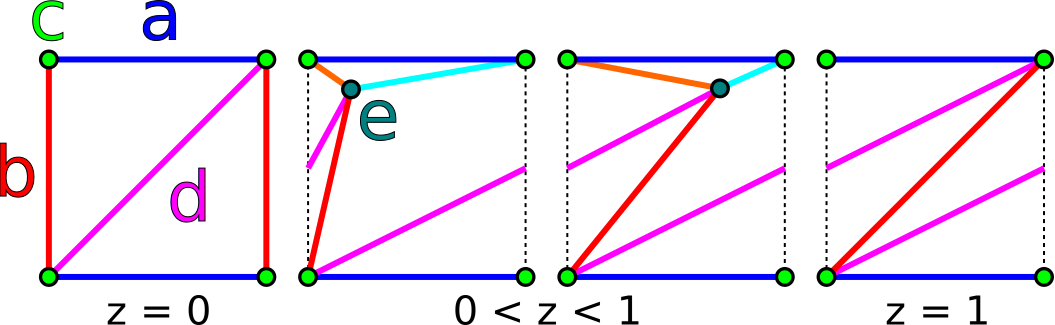
\includegraphics[width = 4in]{_generated/slicesDelta.pdf}
\end{figure}

Now, instead of having a 1-cell \(e\) running across a face, we separate it by a region that resembles a triangular cylinder with pinched top and bottom.
Using this triangulation will give us the same result for \(\pi_1(M)\).
